% 
% Annual Cognitive Science Conference
% Sample LaTeX Paper -- Proceedings Format
% 

% Original : Ashwin Ram (ashwin@cc.gatech.edu)       04/01/1994
% Modified : Johanna Moore (jmoore@cs.pitt.edu)      03/17/1995
% Modified : David Noelle (noelle@ucsd.edu)          03/15/1996
% Modified : Pat Langley (langley@cs.stanford.edu)   01/26/1997
% Latex2e corrections by Ramin Charles Nakisa        01/28/1997 
% Modified : Tina Eliassi-Rad (eliassi@cs.wisc.edu)  01/31/1998
% Modified : Trisha Yannuzzi (trisha@ircs.upenn.edu) 12/28/1999 (in process)
% Modified : Mary Ellen Foster (M.E.Foster@ed.ac.uk) 12/11/2000
% Modified : Ken Forbus                              01/23/2004
% Modified : Eli M. Silk (esilk@pitt.edu)            05/24/2005
% Modified: Niels Taatgen (taatgen@cmu.edu) 10/24/2006

%% Change ``a4paper'' in the following line to ``letterpaper'' if you are
%% producing a letter-format document.

\documentclass[10pt,letterpaper]{article}

\usepackage{cogsci}
\usepackage{pslatex}
\usepackage{apacite}
\usepackage{graphicx, caption, subcaption}

\title{A Dream Model: Reactivation and Re-encoding Mechanisms for Sleep-dependent Memory Consolidation}
 
\author{{\large \bf George Kachergis$^{1}$ (george.kachergis@nyu.edu)} \\
 {\large \bf Roy de Kleijn$^{2}$ (kleijnrde@fsw.leidenuniv.nl)} \\
 {\large \bf Bernhard Hommel$^{2}$ (hommel@fsw.leidenuniv.nl)} \\
  $^{1}$Psychology Department, New York University, USA \\
  $^{2}$Institute of Psychology / Leiden Institute for Brain \& Cognition, Leiden University, the Netherlands} 


\begin{document}

\maketitle


\begin{abstract}
We humans spend almost a third of our lives asleep, and there is mounting evidence that sleep not only maintains, but actually improves many of our cognitive functions. Memory consolidation--the process of crystallizing and integrating memories into knowledge and skills--is particularly benefitted by sleep. We survey the evidence that sleep aids memory consolidation in various declarative and implicit tasks and review the basic neurophysiological structure of sleep with a focus on understanding what neural systems are involved. Drawing on machine learning research, we discuss why it might be useful for humans--and robots, perhaps--to have such an offline period for processing, even though humans are clearly capable of learning incrementally, online. Finally, we propose and simulate two mechanisms for use in computational memory models to accomplish sleep-based consolidation via either or both 1) re-encoding knowledge representations and 2) reactivating and strengthening recent memories.

\textbf{Keywords:} 
memory consolidation; sleep; dreaming; hippocampal replay; memory model
\end{abstract}

\vspace{-.3cm}
\section{Introduction}

Researchers have long been confused why people--and many other animals--spend around a third of their lives asleep. Why has nature burdened us with needing to be in such a vulnerable, unproductive state for so long? Hypotheses abound about why we have evolved to sleep, ranging from it allows us to conserve energy (during a night full of terrors, even), to it simply being a necessary restorative for tired muscles and minds \cite{Siegel:2013}. Both of these example hypotheses are both reasonable and hard to refute (especially the former). Evidence in favor of the latter has been mounting: in a wide variety of cognitive and motoric tasks, performance drops when sleep patterns are interrupted. 

Not only does sleep deprivation cause performance deficits, but there is now substantial empirical evidence that both declarative (i.e., facts and events--`what', `where', `when') and procedural (i.e., skills--`how') memory benefit from even short periods of sleep. Memory is typically described as three processes: 1) encoding: forming new traces from experience, 2) consolidation: integrating memories with prior knowledge and strengthening/crystallizing the trace, and 3) retrieval: task-dependent extraction of overall familiarity or recall of particular traces. Sleep is generally accepted to aid in consolidation, but under what particular circumstances it helps is not fully understood \cite[for a review]{Diekelmann:2009}, nor by which mechanisms it works. 

It is our goal to hypothesize several mechanisms by which sleep could serve to improve consolidation, and to evaluate which of these are suggested by existing empirical evidence. We will begin by considering the computational advantages and disadvantages of online (i.e., incremental; awake) learning versus offline (i.e., batch; asleep) learning, with intuitions imported from the machine learning literature. By considering the often-competing computational needs of the mind (e.g., to quickly and accurately store new information, but also to integrate such episodes with existing knowledge), we hope to better organize existing findings for rational analysis. Thus, we then proceed to review the physiological characteristics of sleep, along with some of the diverse memory effects that have been found. Typical studies often have a similar design (but different task) to the first one that found a benefit for sleep: \citeA{Jenkins:1924} found improved retention of nonsense syllables after a night of sleep as compared to the same amount of time spent awake. However, more recent studies have looked at shorter periods of sleep and also measured the time spent in different sleep stages, which exhibit different types of neural activity. After synthesizing the empirical results, we offer the beginnings of a computational approach to modeling memory consolidation. Despite the large amount of interest in developing computational models of episodic memory \cite[e.g.]{Hintzman:1984,Shiffrin:1997} and semantic memory \cite[e.g.]{Jones:2007}, these models do not yet incorporate sleep-based consolidation mechanisms. We offer several suggestions for concrete changes to an existing model of episodic memory.
\vspace{-.1cm}
\section{Computational Issues}
\vspace{-.1cm}
Machine learning algorithms can be classified as either incremental--allowing data to be added to the model instance by instance--or batch, requiring a (sometimes large) set of training instances before before the model produces useful predictions. Before we dive into a high-level discussion of costs and benefits to these two approaches, let us consider a motivating example. 
\vspace{-.1cm}
\subsection{A Tale of Two Robots}
\vspace{-.1cm}
Imagine two cooking robots running two different versions of the same underlying learning algorithm during a week of daily training to become pizza chefs: Bob runs a batch version, and Ingrid runs an incremental version. Each day, Bob and Ingrid each watch 10 pizzas being made. Bob watches closely, recording every move for processing later that night, whereas Ingrid learns while watching--but is sometimes overwhelmed by too many simultaneous things to pay attention to. On the other hand, even after seeing the first pizza made, Ingrid is able to make predictions about the next, and can evaluate and update her knowledge (and attention to observing particular steps) based on prediction failures. However, by storing all of the input over the day (and perhaps forever), Bob can often make a model that better approximates the real experience than what Ingrid's incremental adjustments add up to. In fact, there may even be particular sequences of experience that can lay a false foundation: for example, consider if Ingrid's first `pizza' experience is a dessert pizza, or `pizza chicken'--not very stereotypical pizzas. For an incremental learner who may hastily build a foundation from the first experience, such a starting point may cause difficulties for focusing on and updating the correct features over the next few recipes experienced. In contrast, Bob's batch algorithm has the advantage of being able to downweight outliers at the end of the day before building his model. Bob's batch and Ingrid's incremental algorithms each have their advantages and disadvantages, and some generalizations are made below.

\subsection{Storage versus Processing}

Incremental or online algorithms (e.g., na\"{\i}ve Bayes) clearly offer the advantage of being able to work (however poorly) with very little data, and can learn immediately when new data are acquired. Moreover, since instances are processed immediately, they do not need to be stored for later updating. One disadvantage is that online updating may require significant computational resources, perhaps at an inconvenient time. In contrast, batch (i.e., offline; e.g., support vector machines, decision trees) learning algorithms may need a large store of data and quite some time to build an initial useful model, and adding a single training instance may require iterating over the entire (and increasing) data store to update the model. A survey of learning algorithms will reveal the classic algorithmic tradeoff: one can store more, and process less upfront (but retrieval can be costly), or process more upfront and store less.

Another problem with many incremental algorithms is the potential to arrive at different learning outcomes based on the order the instances are encountered in. In many cases, such order effects are undesirable, but on the other hand humans and animals show a variety of order effects (e.g., in associative learning: \citeA{Kachergis:2012vc}. Could sleep be a chance to mitigate the order effects brought on during online learning? A few batch-update models have been found to have roughly-equivalent incremental versions. For example, latent semantic analysis \cite[LSA]{Deerwester:1990} learns semantic similarities of words via the singular value decomposition (SVD)--an expensive matrix operation--of a large word $\times$ document co-occurrence matrix. This large matrix--adults know over 70,000 unique words, and have read thousands of documents--must be kept in memory to be updated when a new document is read. Updating the model requires performing the SVD again, so it would be quite expensive to update knowledge every time a new document is read. It is more sensible to read a batch of documents--although, of course, this means that any new knowledge is not available in the model until the latest batch is incorporated. Fortunately, an incremental SVD algorithm has been proposed that not only is less computationally expensive, but also does not require storing the full word $\times$ document \cite{Sarwar:2002}.

Models that use batch updating require storing all of the instances in long-term memory, allowing the model to iterate over all episodes--even multiple times--to extract higher-level features (e.g., correlations of multiple features). On the other hand, incremental updating can reduce the need to store so much information, much of which may be redundant or already over-learned. We conclude that sleep might be a way to get the best of both worlds: incremental learning based on salient features for immediate use, in addition to storage of daily episodes--especially exciting or confusing memories--that can be replayed during sleep to make more thorough, careful updates to knowledge representations before further compressing the memories.

\vspace{-.1cm}
\section{Effects of Sleep}
\vspace{-.1cm}

After a brief summary of the neurophysiological characteristics of sleep, we survey sleep effects found in various declarative and implicit memory tasks.


\subsection{Structure of Sleep}

Sleep in mammals and birds consists of cycles of four stages, proceeding from non-rapid eye movement (NREM) stages 1, 2, and 3 (also called slow-wave sleep), to rapid eye movement (REM) sleep. Human adults typically go through four or five cycles each night, reaching REM sleep every 90 minutes or so. More slow-wave sleep (SWS; NREM3) occurs early in the night, whereas more REM sleep occurs in the last few hours of a night's sleep. Each stage is characterized by particular muscle behaviors and brain activity \cite{Schulz:2008}. 

NREM1, between wakefulness and sleep, is recognized by somewhat active muscles (e.g., fluttering eyelids and rolling eyes) and alpha waves (7.5-12.5 Hz)--as in an awake state--transitioning to a theta rhythm (6-10 Hz). 

NREM2 exhibits lower muscle activity and no awareness of surroundings, as well as a theta rhythm (6-10 Hz), with periodic sleep spindles (11-16 Hz) and K-complexes. It is thought that sleep spindles reflect the brain inhibiting processing, thereby keeping the sleeper asleep, and occur as a result of information flow between thalamic and cortical areas. Sleep spindles often occur together with K-complexes, which are basically delta waves lasting around one second. Their function is thought to be stimulus suppression as well as memory consolidation support.

Sleepers in SWS (NREM3) show very little reactivity to environmental stimuli, and predominantly delta wave activity ($<3.5$ Hz, high amplitude). SWS (i.e. deep sleep) is also when parasomnias such as sleepwalking and night terrors occur. This is the hardest part of sleep to wake up from, and sleep interruption during this stage often lead to feeling groggy and sleepy. There is evidence to suggest that this is an essential stage of sleep: after sleep deprivation, the amount of SWS increases drastically.

Additionally, REM sleep is characterized by rapid, random eye movements as well as most memorable dreaming. At the same time, muscle ationa prevents dreamers from acting out their dreams. Similar to SWS, deprivation of REM sleep increases the amount of REM sleep in a recovery period, indicating that REM is crucial for normal functioning. From neural recordings of rats, it appears that memory replay during non-REM sleep occurs at a 10x speedup, whereas REM replay is roughly at the speed of the behavioral episode \cite{Bendor:2012}. During non-REM sleep, replay happens during short periods of increased activity in cortex and hippocampus related to cortical `up-states' (i.e., frames). Both cortex and hippocampus replay similar content, but replay is initiated in the hippocampus, whereas cortical frames start roughly 50ms before hippocampal frame, leading researchers to conclude that the replay of sequential event memories may be driven by hippocampus, though the memories may be selected by cortex \cite{Lee:2002}.

One of the neurotransmitters that is often studied in relation to memory (especially Alzheimer's disease) and sleep is acetylcholine (ACh). ACh levels are lower during sleep than during awake, except during REM sleep when it reaches higher than awake levels. \citeA{Hasselmo:1999} postulates that ACh inhibits feedback loops within the hippocampus and from it to the neocortex). This means that high ACh levels during waking hours (and REM) supports encoding new declarative memories, whereas low ACh during SWS allows replay of hippocampal memories, which are then stored more permanently in the neocortex.


\subsection{Implicit Memory}

Implicit or non-declarative memories are memories we do not have conscious access to, such as motor skills and procedural and perceptual memory. A positive influence of sleep on a finger tapping task has been demonstrated by \citeA{Walker:2002}, which found that subjects performed 20\% better after a night of sleep compared to subjects spending an equivalent amount of time awake. Furthermore, a correlation was found between the amount of stage 2 NREM sleep and performance improvement. The spindles that are characteristic of stage 2 sleep are thought to trigger specific intracellular mechanisms required for neural plasticity \cite{Walker:2006}. More evidence for this specific influence of stage 2 NREM sleep comes from selective sleep deprivation studies. \citeA{Smith:1994} found worse retention of a visuomotor adaptation task after stage 2 NREM sleep deprivation compared to REM sleep deprivation.

Similar spindles are visible in the somatosensory cortex of newborn rats and humans following spontaneous twitches during REM sleep, suggesting that learning is taking place in the brain following these movements \cite{Khazipov:2004}. As infants spend relatively more of their sleep time in the REM stage compared to adults, muscle twitching during REM sleep may be a way for the body to build (especially in infants) and reinforce (in adults) specific neural pathways from brain to muscles that are frequently used. This mechanism may simply be a low-level version of a similar mechanism known as motor babbling, which allows infants to build higher-level action-effect associations.

Although most sleep-based consolidation studies have used implicit memory tasks, several have been done with declarative memory tasks.

\subsection{Declarative Memory}

The type of memory most people are familiar with is declarative or explicit memory. This type of memory provides us with knowledge of facts, such as Athens being the capital of Greece (semantic knowledge), as well as knowledge of personal events, like what you had for dinner last night (episodic knowledge). 

Declarative memory is thought to be largely dependent on the hippocampus. Evidence supporting this theory consist of patient studies as well as various lesion studies in rats. One famous case includes memory disorder patient H.M., who was unable to form episodic memories after surgery removing a large part of his hippocampus. In rats, Eichenbaum (1990) showed that rats with hippocampal system lesions are severely impaired in the flexible use of previously learned information--normally attributed to episodic memory.

But what is exactly the mechanism by which the hippocampus performs this task? The prevailing hypothesis is that the hippocampus enables the consolidation of memory--i.e., converting an initial memory trace to a stable representation. Sleep is thought to play an important role in memory consolidation, for both declarative and implicit memory. During SWS, the episodic information that is stored in the hippocampus is replayed and projected to brain regions in the neocortex, which stores stable, permanent memories. The direction of this information flow reverses during the REM sleep that occurs later in time. It has been proposed that this allows the hippocampus to remove the unstable, short-term memories in order to make room for new memories to be stored there \cite{Wamsley:2011}.

Indeed, there are many studies showing that sleep improves declarative memory using several paradigms. Retention of nonsense syllables has been shown to improve with sleep since \cite{Jenkins:1924}, and more recent research has shown improvement on a paired associates word list after SWS-rich sleep \cite{Gais:2004}. 

In fact, it seems that not only sleep, but dreaming specifically can have beneficial effects on declarative memory. \citeA{Wamsley:2010} showed that after training on a virtual navigation task, improved performance at retest was correlated with relevant dream imagery during an afternoon nap. Similar thoughts during wakefulness, however, were not correlated with improved performance. It seems that reactivation of recently formed memories facilitates memory consolidation, with dream imagery reflecting this process. Although recall shows more consistent sleep-related benefits than recognition, declarative memory often shows benefits even after only one to two hours of sleep \cite{Diekelmann:2009}. Consolidation of declarative memories has been found to depend more on early hours of sleep, perhaps due to the dominance of SWS, and nondeclarative memory was more aided by the late, REM-dominated hours of sleep \cite{Plihal:1999}.  \citeA{Lee:2002} ran rats repeatedly through a sequence of spatial receptive fields of hippocampal CA1 place cells, and during slow wave sleep (SWS) later ran through the same order of activation at a 20-fold temporal compression of the behavioral sequence, showing that the hippocampus is important for spatial learning--and likely the formation of long-term temporally-extended episodic memories in humans.

In general, SWS seems to aid declarative memory whereas REM enhances procedural and emotional memory in many cases \cite{Mednick:2010}. However, in a study using a sequence learning task (the serial response time task), in which subjects were either explicitly told to learn a (repeating) sequence of button presses or learned it implicitly, the subjects learning explicitly improved only in the sleep condition, and to an extent that was correlated with the amount of NREM sleep \cite{Robertson:2004}. More intriguing was the fact that implicit learners all improved--regardless of sleep--over a twelve hour period, but not after only 15 minutes. Thus, it may be that for procedural memories, intentionally encoded memories are consolidated during sleep, whereas implicit memory consolidation may simply require time.
\vspace{-.1cm}
\section{Theories of Sleep and Dreaming}
\vspace{-.1cm}
An early attempt to explain why we dream was the activation-synthesis hypothesis \cite{Hobson:1977}, which posits that dreams come from the cortex trying to make sense of the random noise produced in the brainstem during REM sleep. We now know that dreaming also occurs during non-REM sleep, and even in deep, `slow-wave' sleep.

\citeA{Walker:2005} proposes that there is a two-phase process by which memories are consolidated during sleep. The hippocampus, which stores recent episodic memories replays events during slow-wave sleep for the neocortex, where long-term memories reside. The communication between the two brain areas at this time is one way, from the hippocampus to the neocortex. During the REM dreaming that follows, though, the flow of information flips, from the neocortex back to the hippocampus. Stickgold suggested that once the neocortex connects the new memories to others in storage, it sends a message back to the hippocampus to erase them.

For declarative memory, there are two basic theories of how memory consolidation is improved during sleep: the active hypothesis states that consolidation depends on sleep, whereas the permissive hypothesis views consolidation as a time-dependent, interference-sensitive process that uses periods of low hippocampus input to process prior information \cite{Mednick:2010}. Procedural memory is just generally thought to be `enhanced' by sleep, but this idea is not universally accepted \cite{Mednick:2010}. An early neural model found that offline replay helped maintain declarative memories using hippocampal-neocortical interplay \cite{Kali:2004}. We will focus on proposing specific computational mechanisms for improving declarative memory, since the current models are more readily adapted to this task, and the empirical evidence indicating the necessity for this is strong.

\vspace{-.2cm}
\section{Model}
\vspace{-.1cm}
Here we will propose and test two mechanisms of sleep-based consolidation that can be added to modern computational models of episodic memory. Our modifications will be specified in terms of the REM\footnote{In this section, REM refers only to the model.} (Retrieving Effectively from Memory) model \citeA{Shiffrin:1997}, which is a multitrace memory model that makes optimal recognition decisions assuming that memory is subject to noise. In multitrace memory models, a memory trace is represented by a large vector of feature values representing the context and content of the event. Some features may be abstract and learned, whereas others are assumed to be simple and sensory-based (i.e., primitive). REM has both episodic traces as well as lexical-semantic traces, the latter of which are de-contextualized accumulations of the various episodic traces, updated across a lifetime. In REM, individual traces are assigned random feature values, each drawn from a geometric distribution with parameter $g$. That is, the probability that a feature has value $v$ is
\begin{equation} \label{eq:geomdist}
P(v) = g(1-g)^{v-1}
\end{equation}
The geometric distribution makes small feature values more probable (and thus frequent) than large values. REM uses these varying base rates in calculating evidence for a memory match: matching a low (common) feature value is not as strong evidence as matching a high value. Conscious experience activates the lexical-semantic (LS) trace for the attended stimuli and updates it with the current context features. An episodic memory trace is formed by copying context and LS features with probability $u$ per time unit $t$. When a feature is stored, it is only copied correctly with probability $c$; otherwise, a random value is drawn according to Equation~\ref{eq:geomdist}. Missing features have a value of 0 (uninformative). Our first proposed modification is to update lexical-semantic (LS) features (i.e., neocortical representations) during a sleep period, when episodic traces since the last sleep period are (randomly, although it may be more accurate to prioritize surprising or emotionally-charged traces) reactivated. The detailed lexical re-encoding mechanism is described in detail below. Updating LS features during sleep leaves the hippocampal episodic traces available for retrieval and recognition throughout the day. REM assumes that when the same stimuli appear multiple times in similar contexts, the old trace may be updated by filling in missing features from LS traces, instead of making a new trace (this differentiation process is how it accounts for the word frequency mirror effect and null list strength effect).

Retrieval in REM uses context features--reinstated by the probe, whatever its source (internal or external)--to activate a subset of long-term memory (e.g., to the studied list of items). This is in part done for simplicity of simulation--so that a number of extra-experimental parameters and processes need not be assumed, but is also a reasonable thing to expect from memory. For recognition, REM computes a likelihood ratio indicating how well test cue $j$ (from the LS traces) match each episodic trace $i$ in the activated subset being considered. This likelihood ratio, in which $g_{sys}$ is the base rate in the long-term, $n_q$ and $n_m$ are the number of non-zero mismatching and matching features, respectively, is defined
\begin{equation} \label{eq:remlik}
\lambda_{i,j} = (1-c)^{n_q} \prod_{v=1}^{\infty} \Big[ \frac{ c + (1-c) g_{sys} \cdot (1-g_{sys})^{v-1} }{ g_{sys}(1-g_{sys})^{v-1} } \Big] ^{n_{m}}
\end{equation}
Thus, the decision depends on not only the number of matching features, but also on how diagnostic the features are: large values are more rare in the geometric distribution, and are thus more informative. Therefore, prior knowledge about the base rate of different values ($g_{sys}$) may affect recognition. REM decides that cue $j$ was presented on the list if the average of the likelihood ratios is above a criterion; else it is rejected. Since small feature values will tend to be quite common and thus undiagnostic, whereas the more useful large feature values are rarely encountered, a potential mechanism for improving memory would be to redistribute feature values. By choosing one or more unique, diagnostic features for each trace (or set of highly-related traces), memory will be improved. Although an exhaustive cross-check to make sure features are unique would be quite computationally expensive (which is why it should be offline), but a simple, greedy version might work well, with high probability. We now describe and test two consolidation methods that we have hinted at.
\vspace{-.1cm}
\section{Simulation}
\vspace{-.1cm}
Using REM as the basis for storing and retrieving memories, we define and test two sleep-based consolidation mechanisms in a simulation of studying 100 items 1, 3, or 5 times\footnote{\texttt{https://github.com/kachergis/REM\_consolidation}}. The \emph{reactivation method} simply reactivates $n$ (here, $n=50$) random memory traces from the day, and then for each of these memories $m$ finds the best matching LS trace $t$ and copies in missing (0-valued) features from $t$ to $m$. In essence, the reactivation mechanism assumes that people dream about recent memories and fill in missing details in the traces using background knowledge. Although these traces are strengthened, the underlying knowledge representations (the LS traces) remain static. In contrast, the \emph{re-encoding method} randomly selects $r$ LS traces (here, $r=50$) for re-encoding, with probability proportional to their familiarity in recent memory (here, the day). For each of these $r$ LS traces, $f$ features (here, $f=6$) are randomly chosen, and those feature values are incremented by 1, thus making those features more diagnostic, and the item easier to remember in the future. However, now that the LS (i.e., neocortical) representation has changed, memories that were encoded with the old representation will be more difficult to retrieve. This can be largely remedied by probing memory for copies of the old representation while re-encoding, and updating those items in memory, as well: simply increment whatever is stored for those $f$ features. Figure~\ref{fig:sleep_sim} shows the mean $d'$ ($z(H) - z(FA)$) of 50 simulated subjects after studying 100 items one, three, or five times, using REM alone or either of the proposed consolidation mechanisms, both of which aid memory. Note that these two methods are complementary, and could be used together with greater effect. The effect of reactivation lessens with more item repetitions, while the re-encoding effect can be quite strong, regardless of repetitions.

%The SARKAE (Storing And Retrieving Knowledge And Events) model \cite{Nelson:2013} develops REM further into a framework that explains how knowledge co-evolves along with episodic memory. Unlike those in REM's traces, the SARKAE's traces represent not only feature values but counts of each feature value (e.g., ``blue") organized by feature types (e.g., ``color"). Event traces contain a single feature value (with a count of 1) if the value is copied from the stimulus, but a feature count vector may instead be copied from memory. Knowledge traces are simply those event traces that have been reactivated and updated many times, and thus contain distributions of feature values. In the SARKAE framework, a straightforward role for sleep is to act as the cleanup period: event traces from the day are considered in turn, and the feature counts of each are either added to an existing knowledge trace (in cortex) if a similar enough one is found, or copied as a new knowledge trace. 
\vspace{-.2cm}
\begin{figure}[!h]
  \centering
  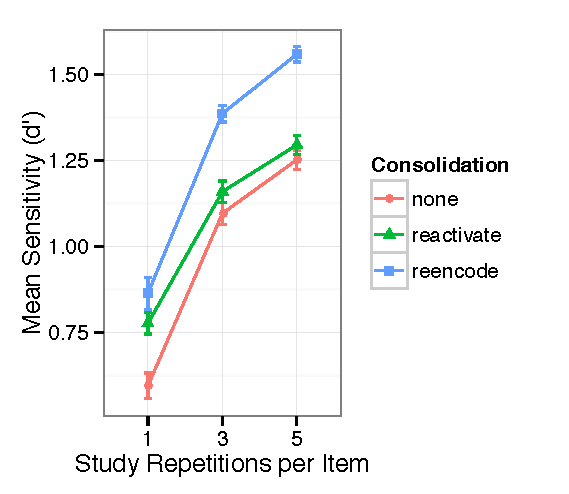
\includegraphics[width=0.36\textwidth]{final_graph_dist1_50reps}
  \caption{Mean $d'$ for REM simulations using no consolidation, or one of reactivation- or re-encoding-based consolidation after studying 100 items 1, 3, or 5 times. Error bars show +/-1SE for 50 simulated subjects.}
  \label{fig:sleep_sim}
\end{figure} 
\vspace{-.2cm}
Variations of these two methods are quite plausible for modeling sleep-based consolidation in current memory models. However, at least one important aspect is clearly missing: structured sequences of events must be linked in some way, but are not in the REM framework (what defines an `event' is not yet known). Future models should address how event boundaries are marked. It may be possible--and would be desirable, for compression--to identify routine sequences (e.g., eating your typical breakfast, or driving home from work via your usual route) and to replace the specific feature values in traces containing these sequences with placeholders pointing to the appropriate LS representation, thus simplifying future updating. Modeling procedural sleep-consolidation effects may require distributed neural models such as \citeA{Kachergis:2014}.
\vspace{-.2cm}
\section{Discussion}
\vspace{-.1cm}
We have proposed two computational mechanisms that could beneficially operate on memories during sleep, along with a rationale for why humans may find it advantageous to be capable of learning by both incremental and batch updating. The proposed mechanisms are all fairly computationally expensive--involving many comparisons and updates to long-term lexical-semantic traces that are presumably stored in neocortex, making them suitable for conducting during sleep. Note that while a complex version of redistributing diagnostic feature values would have to be done in batch, the simple greedy version used here (choosing random features to increment) is more batch-incremental. Although we specified these mechanisms in terms of the REM \cite{Shiffrin:1997} model, the same mechanisms could be used in related multitrace modeling frameworks such as SARKAE \cite{Nelson:2013} or MINERVA2 \cite{Hintzman:1984}. We proposed the reactivation and re-encoding mechanisms based on our survey of sleep-related effects on a variety of declarative and procedural tasks, which we found to convincingly implicate sleep as beneficial to memory consolidation. Our modeling confirms that the proposed methods benefit memory, and offers an avenue for both predicting and matching detailed results from sleep studies. 



%	\begin{table}[!ht]
%	\begin{center} 
%	\caption{Sample table title.} 
%	\label{sample-table} 
%	\vskip 0.12in
%	\begin{tabular}{ll} 
%	\hline
%	Error type    &  Example \\
%	\hline
%	Take smaller        &   63 - 44 = 21 \\
%	Always borrow~~~~   &   96 - 42 = 34 \\
%	0 - N = N           &   70 - 47 = 37 \\
%	0 - N = 0           &   70 - 47 = 30 \\
%	\hline
%	\end{tabular} 
%	\end{center} 
%	\end{table}


%	\begin{figure}[ht]
%	\begin{center}
%	\fbox{CoGNiTiVe ScIeNcE}
%	\end{center}
%	\caption{This is a figure.} 
%	\label{sample-figure}
%	\end{figure}
\vspace{-.2cm}
\section{Acknowledgments}
\vspace{-.2cm}
The preparation of this work was supported by the European Commission (EU Cognitive Systems project ROBOHOW.COG; FP7-ICT-2011).
\vspace{-.2cm}

%\section{References}

\bibliographystyle{apacite}

\setlength{\bibleftmargin}{.125in}
\setlength{\bibindent}{-\bibleftmargin}

\bibliography{holo_sleep_refs}


\end{document}
